\documentclass[a4paper 12pts]{article}
\usepackage[utf8]{inputenc}
\usepackage[T1]{fontenc}
\usepackage[francais]{babel}
\usepackage{graphicx}


\title{Rapport de Projet : iRover}

%mettez vos noms svp !!

\author{R. Joachim CLAYTON, efzefzfzefezfef}

\begin{document}

\maketitle


\begin{figure}[h]
   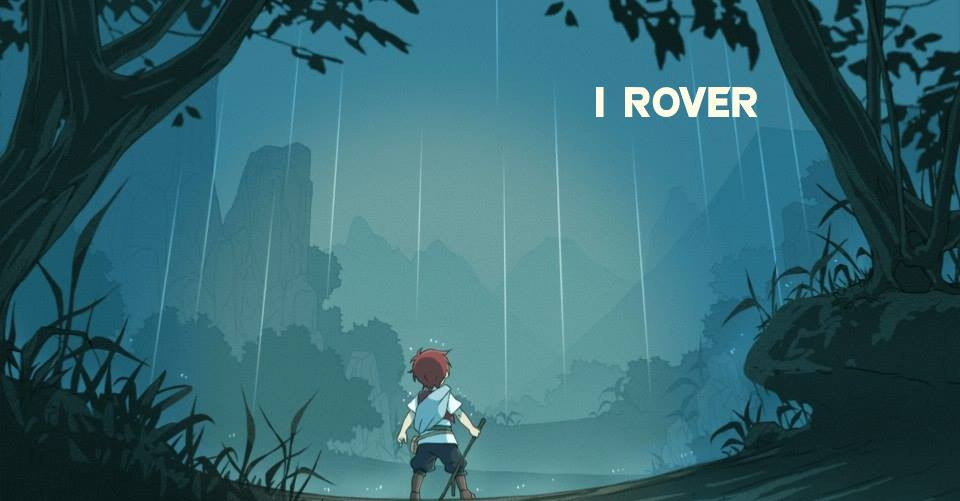
\includegraphics[width=350pt]{Illustration/proj_irover.jpg}
	\caption{iRover, l'histoire d'un héros qu'on appellait robot}
\end{figure}



\newpage


\renewcommand{\contentsname}{Sommaire} 
\tableofcontents

\newpage








\section{Rapport de Projet}


\vspace{2cm}



\subsection{Introduction}
\subsection{Membre du groupe et tâches de chacun}


\section{Définition de la Carte}

%partie de clément


\section{Définition du robot}

%partie Geoff


\subsection{Le robot}
\subsection{Les ennemis}
\subsection{Les coffres}
\subsection{Les clé}
\subsection{La gestion des évênements}
\subsubsection {Rencontre avec un ennemi} 
\subsubsection {Ouvertude d'un coffre}
\subsubsection {Ramasser une clé}

\section{IHM}



\section{IA}

%partie JC

\subsection{path finding}
\subsection{découverte de la carte}



\section{Problèmes rencontrer}

\section{Conclusion}



\end{document}

